\chapter{Collective Grammar and the Emergence of Structural Growth}\label{ch:growth}

This chapter defines the dynamical system studied in the volume and proves its first laws: the orbit is well defined, the fibre only grows, the orbit moves along an integer progression between growth events, each growth event occurs within an explicit number of steps, and consequently the fibre grows without bound.

\section{The collective map and its arithmetic frame}

Throughout, a \emph{realised} value is a positive rational \(x=a/b\) in lowest terms with \(\Dx(x)\ne\varnothing\), where \(\Dx(x)=\{d\ge2: d^2\mid a,\ d\equiv1\ (\mathrm{mod}\ b)\}\). Write \(R(x)=|\Dx(x)|\), \(L(x)=\lcmop\Dx(x)\), \(G(x)=\gcd\{d-1:d\in\Dx(x)\}\).

\begin{definition}[The collective map]\rec{F.CDEF}\scope{C}
For a realised value \(x\) put
\[
\Dcoll(x)=\frac{L(x)^2}{G(x)},\qquad C(x)=x+\Dcoll(x).
\]
The \emph{collective orbit} of a realised \(x_0\) is \(x_{n+1}=C(x_n)\). Write \(\Dx_n,R_n,L_n,G_n\) for the quantities of \(x_n\), and \(\gamma(x)=x/\Dcoll(x)\).
\end{definition}

By Volume~I (Theorem~2.5), \(x+j\Dcoll(x)\) (\(j\ge0\)) are exactly the values shared by all routes through \(x\) at or after \(x\). The map \(C\) selects \(j=1\): the first collective meeting. The definition is an adopted interaction rule; Volume~I proved that the arithmetic leaves this choice open. The theorems below concern what the adopted rule does. The next proposition fixes the arithmetic frame in which every later statement is written; it uses nothing but the definition of \(\Dx\).

\begin{proposition}[The collective step is reduced and \(\gamma\) is an integer]\rec{F.T17p}\scope{A0}\label{prop:frame}
Let \(x=a/b\) be realised, \(G=G(x)\), \(L=L(x)\). Then
\begin{enumerate}[label=(\alph*),nosep]
\item \(b\mid G\);
\item \(\gcd(L,G)=1\); hence \(\Dcoll=L^2/G\) is in lowest terms and has denominator \(G\);
\item \(L^2\mid a\); the number \(y=Gx=aG/b\) is an integer divisible by \(L^2\), and \(\gamma(x)=y/L^2\) is a positive integer. Thus \(x=\gamma L^2/G\).
\end{enumerate}
\end{proposition}
\begin{proof}
(a) Each \(d\in\Dx\) satisfies \(b\mid d-1\), so \(b\mid G\). (b) A prime \(p\mid G\) divides \(d-1\) for every \(d\in\Dx\), hence divides no \(d\), hence not \(L\). (c) \(d^2\mid a\) for all \(d\in\Dx\) gives \(L^2=\lcmop(d^2)\mid a\). By (a), \(G/b\) is an integer, so \(y=a\,(G/b)\) is an integer divisible by \(L^2\). Finally \(\gamma=x/\Dcoll=Gx/L^2=y/L^2\).
\end{proof}

\begin{theorem}[Monotone orbits]\rec{F.T31}\scope{C}\label{thm:mono}
For every realised \(x\): \(\Dx(x)\subseteq\Dx(C(x))\) and \(G(C(x))\mid G(x)\). Consequently every collective orbit is defined for all \(n\), \(\Dx_n\subseteq\Dx_{n+1}\), and \(G_{n+1}\mid G_n\).
\end{theorem}
\begin{proof}
Let \(x=a/b\), \(G=G(x)\), \(L=L(x)\). Over the denominator \(G\) the value \(x'=C(x)\) is \(N/G\) with \(N=a(G/b)+L^2\). Take \(d\in\Dx(x)\). Then \(d^2\mid a\), so \(d^2\mid a(G/b)\); also \(d^2\mid L^2\); hence \(d^2\mid N\). Since \(G\mid d-1\), we have \(\gcd(d,G)=1\), so \(d^2\) divides the numerator of \(N/G\) in lowest terms, and \(d\equiv1\) modulo \(G\), hence modulo the reduced denominator, a divisor of \(G\). Thus \(d\in\Dx(x')\). The gcd defining \(G(x')\) runs over a larger set, so \(G(x')\mid G(x)\). Inductively every \(x_n\) is realised.
\end{proof}

\section{Plateaus and the time to the next growth}

Between growth events the data \((\Dx,L,G)\) are constant and the orbit moves along an arithmetic progression.

\begin{proposition}[Plateau law]\rec{F.T17}\scope{C}\label{prop:plateau}
Suppose \(\Dx_{n_0+k}=\Dx_{n_0}\) for \(0\le k\le K\). Then \(x_{n_0+k}=(\gamma_{n_0}+k)\,L^2/G\) and \(\gamma_{n_0+k}=\gamma_{n_0}+k\) for \(0\le k\le K\).
\end{proposition}
\begin{proof}
\(L\) and \(G\) are constant on the plateau, so \(x_{n_0+k}=x_{n_0}+k\Dcoll\), and dividing by \(\Dcoll\) gives \(\gamma\) increasing by one per step.
\end{proof}

Write \(T(x)\) for the least \(n\ge1\) with \(\Dx(C^n(x))\ne\Dx(x)\), the time to the next growth. It is finite by the next theorem.

\begin{theorem}[Growth-time bound]\rec{F.T18}\scope{C}\label{thm:growth-time}
Let \(x\) be realised, \(\gamma=\gamma(x)\), \(G=G(x)\), and let \(d\ge2\) be an integer with \(d\notin\Dx(x)\). Put
\[
K_d=Gd^2\Big\lceil\frac{\gamma}{Gd^2}\Big\rceil-\gamma .
\]
Then \(1\le K_d\le Gd^2-1\) and \(T(x)\le K_d\). In particular \(T(x)\le G\,d_{\min}^2-1\), where \(d_{\min}\) is the least integer \(\ge2\) not in \(\Dx(x)\).
\end{theorem}
\begin{proof}
The ceiling gives \(0\le K_d<Gd^2\). If \(K_d=0\), then \(Gd^2\mid\gamma\), so \(x=\gamma L^2/G=(\gamma/G)L^2\) is an integer divisible by \(d^2\), whence \(d\in\Dx(x)\) (a modulus condition modulo \(b=1\) is empty): a contradiction. So \(K_d\ge1\). Suppose no growth occurs in the steps \(1,\dots,K_d\). By Proposition~\ref{prop:plateau}, \(x_{K_d}=(\gamma+K_d)L^2/G=d^2\lceil\gamma/(Gd^2)\rceil L^2\), an integer divisible by \(d^2\). Then \(d\in\Dx(x_{K_d})=\Dx(x)\), contradicting \(d\notin\Dx(x)\).
\end{proof}

The bound is an upper bound; actual growth is usually earlier because several moduli may become available at once. Its best form over all choices of \(d\) is computable by a finite search.

\begin{proposition}[Exact minimum of the bound]\rec{F.T26}\scope{C}\label{prop:minK}
Let \(k_0=K_{d_{\min}}\). Then \(\min\{K_d:d\ge2,\,d\notin\Dx(x)\}\) is attained at some \(d\) with \(d^2<(\gamma+k_0)/G\) (or equals \(k_0\)); hence it is computed by a finite search, and \(T(x)\) is at most this minimum.
\end{proposition}
\begin{proof}
If \(K_d<k_0\), then \(Gd^2\le Gd^2\lceil\gamma/(Gd^2)\rceil=\gamma+K_d<\gamma+k_0\), because \(\gamma\ge1\). Hence only \(d\) with \(Gd^2<\gamma+k_0\) can improve on \(k_0\).
\end{proof}

\begin{example}\label{ex:orbit36}
The orbit of \(x_0=36\) has \(\Dx=\{2,3,6\}\), \(G=1\), \(L=6\), \(\Dcoll=36\) and runs \(36,72,108\) with \(\gamma=1,2,3\); at \(144\) the modulus \(4\) (and with it \(12\)) appears. The orbit of the natural seed \(x_0=45828/5\) has \(\Dx=\{6\}\), \(G=5\), \(\gamma_0=1273\), and acquires the moduli \(21\), \(126\), \(36,\dots\) within three steps:
\begin{center}\small
\begin{tabular}{r|rrrrrrrrr}
\(n\) & 0 & 1 & 2 & 3 & 4 & 5 & 6 & 7 & 9\\\hline
\(R(x_n)\) & 1 & 2 & 3 & 4 & 4 & 4 & 5 & 5 & 7\\
\(\gamma_n\) & 1273 & 26 & 3 & 1 & 2 & 3 & 1 & 2 & 1\\
\(L_n\) & 6 & 42 & 126 & 252 & 252 & 252 & 504 & 504 & 1008
\end{tabular}
\end{center}
Here \(G_n=5\) for every \(n\), a persistent regime studied in Chapter~\ref{ch:persist}; the large initial \(\gamma\) falls at the carries \(6\to42\to126\) and the orbit settles into the cycle \(\gamma=1,2,3\) with a carry every third step.
\end{example}

\section{Unbounded generative multiplicity}

\begin{theorem}[Collective fibre growth]\rec{F.T19}\scope{C}\label{thm:growth}
For every realised \(x_0\): \(R(x_n)\) is non-decreasing, \(R(x_n)\to\infty\), and \(\bigcup_n\Dx(x_n)\) is infinite.
\end{theorem}
\begin{proof}
Monotonicity is Theorem~\ref{thm:mono}. By Theorem~\ref{thm:growth-time} every growth event occurs within finitely many steps (for any \(d\notin\Dx(x_n)\), which exists because \(\Dx(x_n)\) is finite), and each event adds at least one modulus to a set that never shrinks. So there are infinitely many events and \(R\) is unbounded; being non-decreasing, it tends to infinity.
\end{proof}

There is no infinite plateau, and no orbit has bounded fibre. The theorem makes no claim about \emph{rate}; the next proposition gives an explicit but weak lower bound, and Chapters~\ref{ch:regimes}--\ref{ch:gamma} determine the true rate in every regime (linear growth of \(R\) in the regimes found).

\begin{proposition}[A provable growth rate]\rec{F.T27}\scope{C}\label{prop:rate}
Let \(v_0=G(x_0)\). (a) \(G(x_n)\le v_0\) for all \(n\). (b) \(d_{\min}(x)\le R(x)+2\). (c) If \(R(x_n)=R\) then \(T(x_n)\le v_0(R+2)^2-1\), and
\[
R(x_n)>\Big(\frac{3n}{v_0}\Big)^{1/3}-3\qquad(n\ge1).
\]
\end{proposition}
\begin{proof}
(a) is Theorem~\ref{thm:mono}. (b) The \(R+1\) integers \(2,\dots,R+2\) cannot all lie in a set of \(R\) elements. (c) Combine (a), (b) and Theorem~\ref{thm:growth-time}. Let \(n(r)\) be the first step with \(R\ge r\). If \(R(x_{n(r)})=r\) then \(n(r+1)\le n(r)+v_0(r+2)^2-1\); otherwise \(n(r+1)=n(r)\). Therefore, if \(R=R(x_n)\), then \(n<n(R+1)\le v_0\sum_{r=1}^{R}(r+2)^2\le v_0(R+3)^3/3\), which is the stated inequality.
\end{proof}

The bound is deliberately weak (the sampled orbits of Figure~\ref{fig:growth} grow linearly), but it is unconditional, and it is the only rate available before the structure of Chapters~\ref{ch:persist}--\ref{ch:schedule} is in place.

\begin{figure}[t]
\centering
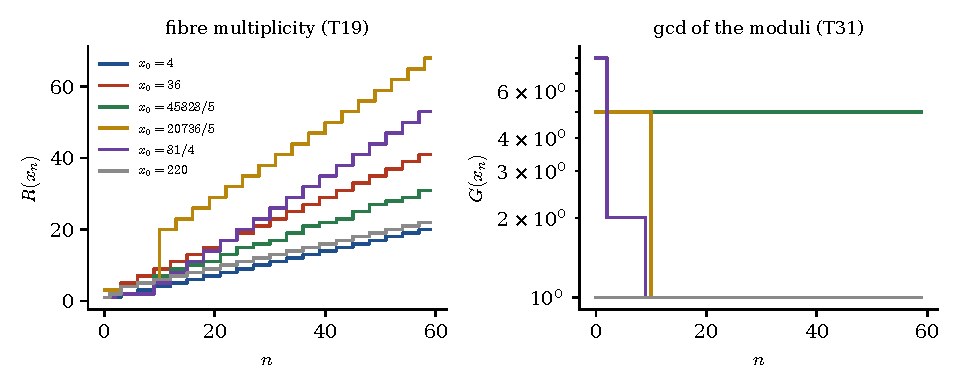
\includegraphics[width=0.97\linewidth]{figs/fig_growth.pdf}
\caption{Collective growth along six exact orbits (60 steps each). Left: \(R(x_n)\), non-decreasing and unbounded (Theorem~\ref{th:F.T19}). Right: \(G(x_n)\), which can only drop through divisors (Theorem~\ref{th:F.T31}). The orbits from \(4\), \(36\), \(220\) have \(G=1\) throughout; \(20736/5\) (from \(G=5\)) and \(81/4\) (from \(G=8\)) collapse to \(G=1\); the orbit from \(45828/5\) stays at \(G=5\) for all 60 steps.}\label{fig:growth}
\end{figure}

\section{Growth is specific to the collective branch}

The monotonicity of the fibre is not a property of the arithmetic progression through a value; it is a property of the \emph{collective} step, which advances by the common difference of the whole fibre.

\begin{example}[Route-aware continuation does not preserve the fibre]\rec{F.T28}\scope{C}\label{ex:T28}
Take \(x=36\) with the pair of routes \((2,3)\), whose pairwise common-future step is \(\Delta=36\) (Volume~I, Theorem~2.2). Along \(x+k\Delta=36(k+1)\) the fibre sizes are
\[
R(36(k+1))=3,3,3,5,3,3,3,5\quad(k=0,\dots,7),
\]
so \(R\) drops from \(5\) to \(3\) at \(180\), whereas along the collective orbit \(\Dx\) never shrinks. (In the corpus, \(R\) decreases within ten steps along the pair orbit in every one of the 118 tested cases; this is data, not a claim.)
\end{example}

The two continuations differ for a precise reason: the collective step is a common multiple of every pairwise step, so each route continues to the new value (Theorem~\ref{thm:mono}), while a pairwise step ignores the routes outside the pair and may leave their progressions.
